\chapter{System Identification} \label{ch:sysid}

The second aspect of this thesis involves modeling the existing controllers operating the fiber drawing plant. Given limited information about the controllers (e.g. their order and sampling time), a time-series statistical analysis approach is used to model each controller and simulate outputs. The theory behind time-series system identification is briefly reviewed in Section \ref{ch:sysid:theory}. Section \ref{ch:sysid:proc} describes the methods and analyses involved in identifying and validating models, as applied to our optical fiber extrusion system. Lastly, the process of identifying the bare fiber diameter controller is presented in Section \ref{ch:sysid:case} as a case study. All analyses were performed using MATLAB R2021b. 

\section{Theory of Data-Based Models} \label{ch:sysid:theory} 

As discussed in Section \ref{ch:ml:relation}, the dynamics of a discrete nonlinear system is a function of the system's past states and inputs, up to some number of timesteps. (Refer to Equation \ref{eqn:nonlinear_discrete}.) Aside from RNNs, there are also data-based models well-suited for time-series prediction and identifying controllers. \cite{armax1, armax2} If given a sufficient amount of input-output data of a system, a model can be developed solely on those data while abstracting away from the equations of motion and the underlying physics. This is the essence behind black-box system identification. It allows for modeling dynamical systems not easily derived from first principles. 

\begin{figure}[t!]
    \begin{center}
        \tikzstyle{ann} = [above, text width=2.5em]
        \def\edgedist{3}
        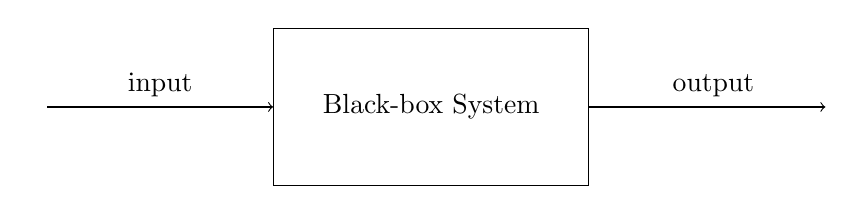
\begin{tikzpicture}
                % draw rectangle node
                \node[draw,
                    minimum width=4cm,
                    minimum height=2cm] (sys) at (0,0) {Black-box System};
                \node[draw=white,
                    minimum width=0cm,
                    minimum height=0cm] (empty) at (-5,0) {};
                % Draw edges
                \draw [->] (sys.east) -- node [ann] {output} + (\edgedist,0);
                \draw [->] (empty.east) -- (sys.west) node[midway,above] {input};
        \end{tikzpicture}
    \end{center}
    \caption{Black-box view of system identification.}
    \label{fig:blackbox}
\end{figure}

System identification has been a well-studied topic in literature. Black-box models have been developed for damping controllers in power grids \cite{smartgrid}, model predictive controllers for car-following \cite{car_following}, static heat flow estimation \cite{static_heat_flow}, just to name a few. It is a widely used and powerful technique to model systems from measured, and often noisy, data. An accurate model of the system is helpful for predicting system outputs from given inputs; such input-output correlations, in turn, guides the design of controllers that enable the system to reach desired performance.

\begin{figure}[b!]
    \centering
    \includegraphics{figures/sys_general.png}
    \caption{General linear model structure for the system identification problem \cite{ni}.}
    \label{fig:sys_general}
\end{figure}

The time-series system identification problem can be posed as follows. Figure \ref{fig:sys_general} illustrates the general discrete-time linear model for a Single-Input, Single-Output (SISO) process. It can be described by the difference equation in Equation \ref{eqn:sysid_general}. 
\begin{equation}
    \label{eqn:sysid_general}
    A(q) y(t) = \frac{B(q)}{F(q)} u(t) + \frac{C(q)}{D(q)} e(t)
\end{equation}
where $u(t)$ is the system input and $y(t)$ the system output. $e(t)$ is the noise signal entering the system and is usually assumed to be white noise. $q$ denotes the \emph{time-shift operator} which, when applied to a signal, advances the signal one timestep ahead. Inversely, applying $q^{-1}$ to a signal shifts the signal backwards by one timestep. Mathematically, 
\begin{equation}
    \label{eqn:def_q}
    \begin{split}
        qu(t) & = u(t+1) \\
        q^{-1}u(t) & = u(t-1)
    \end{split}
\end{equation}

As $A$, $B$, $C$, $D$, and $F$ are defined as polynomials of $q^{-1}$, the system output $y(t)$ at the current timestep is predicted as a function of data from the past timestep(s). Implicit in these model architectures is the assumption of \emph{causality} — the property that outputs depend on the past and current inputs but not future inputs. Specifically, 
\begin{equation}
    \begin{split}
        A(q) &= 1 + a_1 q^{-1} + ... + a_{n_a} q^{-n_a}\\
        B(q) &= b_1 + b_2 q^{-1} + ... +b_{n_b} q^{-n_b+1}\\
        C(q) &= 1 + c_1 q^{-1} + ... + c_{n_c} q^{-n_c}\\
        D(q) &= 1 + d_1 q^{-1} + ... + d_{n_d} q^{-n_d}\\
        F(q) &= 1 + f_1 q^{-1} + ... + f_{n_f} q^{-n_f}
    \end{split}
\end{equation}

In this work, two specific models of the generalized architecture described above are explored: the Output-Error (OE) model, and the AutoRegressive Moving-Average model with eXogenous inputs (ARMAX). The theory behind their architectures is treated in detail in the following subsections. 

\subsection{OE Model}

\begin{figure}[h]
    \centering
    \includegraphics{figures/oe.png}
    \caption{Diagram of the OE model \cite{ni}.}
    \label{fig:oe}
\end{figure}

Figure \ref{fig:oe} illustrates the architecture of the OE model. Its model structure is given by

\begin{equation}
    \label{eqn:oe}
     y(t) = \frac{B(q^{-1})}{F(q^{-1})} u(t-n_k) + e(t)
\end{equation}
where $n_k$ is known as the \emph{input delay}\footnote{Also known as \emph{transport delay} or \emph{dead time}.} of the system, which is the number of input samples that occur before the outputs are affected. The OE model structure describes the system dynamics separately from the noise signal. The polynomial acting upon the noise signal $e(t)$ is unity, which means that the noise entering the system is modeled to be zero-mean white noise, and no other parameters are used to characterize the disturbance. 

\subsection{ARMAX Model}

\begin{figure}[h]
    \centering
    \includegraphics{figures/armax.png}
    \caption{Diagram of the ARMAX model \cite{ni}.}
    \label{fig:armax}
\end{figure}

A diagram of the ARMAX model is depicted in Figure \ref{fig:armax}. Its input-output relation is given by
\begin{equation}
    \label{eqn:armax}
    A(q^{-1}) y(t) = {B(q^{-1})} u(t-n_k) + {C(q^{-1})} e(t)
\end{equation}
where all variables are similarly defined as before. The ARMAX model is no more than the specific case of the general system in Equation \ref{eqn:sysid_general}, with $D$ and $F$ polynomials set to unity. Unlike the OE model, the ARMAX model integrates the disturbance dynamics together with the system dynamics. It is particularly useful due to its assumption that there are prominent disturbances entering at the input and propagating through the system dynamics. The error dynamics is also parametrized by $C(q)$, which indicates that the noise is assumed to be colored. 

\subsection{Implementation in MATLAB}

The parameter estimation process was implemented in MATLAB with its System Identification Toolbox. Given the input-output data of a system (in the form of an \texttt{iddata} object) and specified orders of each polynomial, the toolbox provides functions, such as \texttt{oe(data, orders)} and \texttt{armax(data, orders)}, that perform the model fitting and return a representation of the system as an \texttt{idpoly} object (the MATLAB representation of the generalized system in Figure \ref{fig:sys_general}). 

The identified parameters are the result of an iterative search algorithm, introduced in a paper by Wills et al. \cite{iter_sysid_wills}. The algorithm poses a least squares optimization problem in which the prediction error, i.e. the error between simulated output from the prediction and measured output from the data, is minimized. As proven by Ljung (1999) \cite{ljung1999system}, the general model described by Equation \ref{eqn:sysid_general} is linear in its parameters, therefore it is appropriate to pose the parameter identification problem in the general model as a multi-stage least square problem. MATLAB also has built-in functions to validate identified models, using the normalized root mean square error (NRMSE) as the figure of merit. Namely, for a measured output $y$ with mean $\Bar{y}$ and a prediction output $\hat{y}$, the percentage of accuracy is calculated as, 

\begin{equation}
    \label{eqn:sysid_fit}
    \text{fit} = \left(1-\frac{\left\lVert y-\hat{y}\right\rVert}{\left\lVert y-\Bar{y}\right\rVert}\right) \times 100 \%
\end{equation}

The iterations terminate when the specified maximum number of iterations is reached or the accuracy increment is lower than the specified tolerance. %The validation process for this work will be discussed in full detail in Section \ref{ch:sysid:proc:val}.

\section{System Identification Procedures} \label{ch:sysid:proc}

\begin{figure}[ht!]
    \centering
    \includegraphics[width=0.6\textwidth]{figures/sysid_pipeline.png}
    \caption{Diagram of the system identification pipeline \cite{sysid_pipeline}.}
    \label{fig:sysid_pipeline}
\end{figure}

Introduced by Ljung \cite{ljung1999system}, the system identification method is an iterative process to identify a model with some \emph{a priori} knowledge of the system. In general, given the measured input-output data of a system, the task of system identification can be divided into subproblems as follows: 

\begin{enumerate}
    \item Design and perform experiments to acquire the necessary input-output data 
    \item Specify a proper model structure or a set of candidate model structures 
    \item Select appropriate model orders in the chosen structure(s) based on the principle of parsimony 
    \item Specify a criterion of fit with which the models are evaluated
    \item Identify the model parameters based on the criterion of fit
    \item Validate the model, examine its properties, and simulate system output
    \item If necessary, revisit any of the steps above and iterate forwards to refine the identified system parameters
\end{enumerate}

The following subsections present the details of this process as applied to the controllers in the fiber drawing system. 

\subsection{Model Order Bounds} \label{ch:sysid:proc:order}

Given the potential candidates for model structures, the objective of system identification is to identify the simplest, interpretable model that provides the best fit to the collected data. Especially for controller design, an underestimate of the orders would result in a biased model, whereas an overly high order model would be less reliable, computationally expensive to implement, and would lose its robustness to disturbances. Thus, the order selection process is usually guided by the \emph{principle of parsimony}, which states that the simplest model that can explain the data is to be preferred. In this work, this principle puts preference on an identified system with the lowest maximum order that satisfies the goodness criteria. 

A reasonable estimate of the range of the system's model order can be drawn from first principles of the physical  system. In this work, the systems in question are bare fiber diameter controller and the tension controller within the optical fiber drawing tower. % TODO: submit that paper and cite myself here
Given limited \emph{a priori} knowledge about the system, namely that the controllers in the tower are implemented as PID controllers, one can begin with analytical equations and develop a first-principles model relating the input to the output. 

\begin{figure}[h!]
    \centering
    \includegraphics[width=0.8\textwidth]{figures/pid.png}
    \caption{Block diagram of a PID controller in a feedback loop \cite{pid}.}
    \label{fig:pid}
\end{figure}

The internal schematic of a typical PID controller is shown in Figure \ref{fig:pid}. Let $e(t) = r(t) - y(t)$ be the input signal to the PID controller, and is defined as the deviation of the plant output $y(t)$ from the desired reference signal $r(t)$ that the controller aims to follow. Let $u(t)$ be the control effort, the output of the controller. The control law of a PID controller, expressed in the time domain, is shown in Equation \eqref{eqn:pid}. 

\begin{equation}
    \label{eqn:pid}
    \frac{u(t)}{e(t)} = K_P e(t) + K_I\int_0^T e(t) dt + K_D \frac{d}{dt} e(t)
\end{equation}
where $K_P$, $K_I$, and $K_D$ are the proportional, integral, and derivative gains respectively. 

Let's examine the rate of change in the control effort $u(t)$ in Equation \eqref{eqn:pid_dt}. 

\begin{equation}
    \label{eqn:pid_dt}
    \frac{du}{dt} = K_P \frac{d}{dt} e(t) + K_I e(t) + K_D \frac{d^2}{dt^2} e(t)
\end{equation}

In real-world machinery, derivatives are calculated or approximated by taking the finite difference \cite{finite_diff} between time steps. Thus, Equation \eqref{eqn:pid_dt} can be written as 
\begin{equation}
    \label{eqn:pid_fd}
        \frac{u[n]-u[n-1]}{\Delta t} 
         = K_P \frac{e[n]-e[n-1]}{\Delta t} + K_I e[n] + K_D \frac{e[n]-2e[n-1]+e[n-2]}{\Delta t}
\end{equation}
where $\Delta t$ is the sampling time between discrete measurements. 

To reformulate the above relationship with variables used in Section \ref{ch:sysid:theory} and other series analysis literature, we express the above equation in terms of the time-shift operator $q$ (defined in Equation \ref{eqn:def_q}), 
\begin{equation}
    u-q^{-1}u = K_P e (1-q^{-1}) + K_I e \Delta t + K_D e (1-2q^{-1}+q^{-2})
\end{equation}

Rearranging further, we obtain the transfer function of the PID controller as
\begin{equation}
    G(q) = \frac{u(q)}{e(q)} = \frac{K_P (1-q^{-1}) + K_I \Delta t + K_D (1-q^{-1})^2}{1-q^{-1}}
\end{equation}

\begin{equation}
    G(q) = \frac{(K_P + K_D + K_I\Delta t) - (K_P-2K_D) q^{-1} + K_D q^{-2}}{1-q^{-1}}
\end{equation}

This suggests that a PID controller is at least second order in nature. 

In addition, due to the noisy nature of the measured data (illustrated later in Section \ref{ch:sysid:case}), a low-pass filter of some sort is warranted for controller stability. Such filters introduce at least one order in the system. There may also be unmodeled dynamics in the system that is not captured in this analysis, which, in turn, translates to higher order required for a reasonable fit in system identification. Therefore, we have established a third-order lower bound for the identified model. 

\subsection{The Grid Search} \label{ch:sysid:proc:grid}

For each subbatch (defined in Section \ref{ch:exp:data}), a grid search is implemented to select the model orders. The problem is posed as follows. Consider the OE architecture. Let $\mathcal{S}_{OE} \subseteq \mathbb{N}^3$ denote the parameter search space to be iterated through. The maximum order $N_{max}$ is chosen to be the upper limit of the model order in the search space; in this study it is set to be $10$. $K_{max}$, the upper bound of $n_k$, is set to be $4$. Furthermore, with the lower bound of the order determined above, the goal of the grid search is to select an OE model with orders $[n_a, n_b, n_k]$ where

\begin{equation*}
    (n_a, n_b, n_k)\in \mathcal{S}_{OE} = [1, N_{max}]^2 \times [1, K_{max}] \text{\space\space s.t. } \max(n_a, n_b) \geqslant 3
    \label{eqn:oe_bounds}
\end{equation*}

Additionally, the criteria of fit is enumerated below. A selected candidate OE model should: 

\begin{enumerate}
    \item Perform a reasonable fit to a majority of the subbatches\footnote{A reasonable fit is quantified by a minimum percentage accuracy, here set to be 50\%, as calculated using Equation \ref{eqn:sysid_fit}.\label{ftn:good}}
    \item Attain a satisfactory average accuracy across subbatches of good fit\footnote{Some subbatches of data were discarded due to an impossible fit caused by measurement errors from operator interruption.}
    \item Be characterized by polynomials of low orders per the principle of parsimony discussed in Section \ref{ch:sysid:proc:order}.
\end{enumerate}

Once a set of candidate model orders $[n_a, n_b, n_k]$ are identified, engineering decision is involved to choose a model that balances the three objectives above. The pseudocode summarizing this process is presented in Algorithm \ref{alg:grid_search_oe}. The grid search process for ARMAX is similar; the search space $\mathcal{S}_{ARMAX} \subseteq \mathbb{N}^4$ is iterated through, with the same lower and upper bounds determined above, generating candidate models with orders $[n_a, n_b, n_c, n_k]$ where
\begin{equation*}
    % (\texttt{na}, \texttt{nb}, \texttt{nc})\in \mathcal{S} = [1, N_{max}]^3 \text{\space\space s.t. } \max(\texttt{na}, \texttt{nb}, \texttt{nc}) > 3
    (n_a, n_b, n_c, n_k)\in \mathcal{S}_{ARMAX} = [1, N_{max}]^3 \times [1, K_{max}] \text{\space\space s.t. } \max(n_a, n_b) \geqslant 3
    \label{eqn:armax_bounds}
\end{equation*}

As shown in Algorithm \ref{alg:grid_search_oe}, during the grid search process, the accuracy percentages for all orders for all subbatches are stored for comparison purposes, in a table in which each row is a subbatch and each column is a combination of model orders attempted for the fit. A final model is then selected among the best-performing candidate models, after comparing their number of subbatches with reasonable fits and average accuracies. 

% \begin{algorithm}[p]
%     \label{alg:grid_search_oe}  
%     \DontPrintSemicolon
%     \caption{Grid Search for OE Model Orders.}
%     \KwData{$F$ = A list of files each containing many subbatches of fiber production data within a week.}
%     \KwResult{$M$ = A 2D matrix of fit percentages for all subbatches for all orders.}
%     % \For{each file $f \in F$}{
%     %     \For{each subbatch in $f$}{
%     %         \texttt{iddata\_obj} = \texttt{iddata(capstan\_speed, bfd\_error, sampling\_time)}\;
%     \For{na \in [1, N_{max}]}{
%         \For{nb \in [1, N_{max}]}{
%             \If{\textbf{not } na<3 and nb < 3}{
%                 \texttt{sys\_kd} = \texttt{oe(iddata\_obj, [na, nb, 3])}\;
%                 \texttt{fit\_percentage} = \texttt{compare(iddata\_obj, sys\_kd)}\;
%                 \If{$50 \leq fit\_percentage \leq 100$}{
%                     Store fit\_percentage in $M$\;
%                 }
%             }
%         }
%     }
%     %     }
%     % }
% \end{algorithm}

% % REVISE TO USE ALGORITHM2E PACKAGE... LOOKS NICER

\begin{algorithm}[t]
    \KwData{$F$ = A list of files each containing many subbatches of fiber production data within a week.}
    \KwResult{$M$ = A 2D matrix of fit percentages for all subbatches for all orders.}
    \begin{algorithmic}
        \caption{Grid Search for OE Model Orders.}
        \label{alg:grid_search_oe}
        \FOR{each file $f \in F$}{
            \FOR{each subbatch $\in f$}{
            \STATE \texttt{iddata\_obj} = \texttt{iddata(capstan\_speed, bfd\_error, sampling\_time)}\;
                \FOR{$n_a \in [1, N_{max}]$}{
                    \FOR{$n_b \in [1, N_{max}]$}{
                        \FOR{$n_k \in [1, K_{max}]$}{
                            \IF{$\textbf{not } n_a<3 \And n_b < 3$}{
                                \STATE \texttt{sys\_kd = oe(iddata\_obj, [na, nb, 3])}\;
                                \STATE \texttt{fit\_percentage} = \texttt{compare(iddata\_obj, sys\_kd)}\;
                                \IF{$50 \leqslant \texttt{fit\_percentage} \leqslant 100$}{
                                    \STATE Store \texttt{fit\_percentage} in $M$\;
                                } \ENDIF
                            } \ENDIF
                        }\ENDFOR
                    } \ENDFOR
                }\ENDFOR
            } \ENDFOR
        } \ENDFOR
    \end{algorithmic}
\end{algorithm}

\subsection{Model Validation} \label{ch:sysid:proc:val}

\subsubsection{Frequency-Domain Analysis}

Besides comparing the measured output with predicted output signals in the time domain using Equation \ref{eqn:sysid_fit}, the power spectrum of the output signals and the frequency-domain properties of the control loop should be examined when validating the identified model. The power spectrum of the system output should be compared to that of the predicted output. The prediction should not only capture the low-frequency trends in the output but also agrees reasonably in the high-frequency regime. It is important to identify the frequency ranges in which the prediction performs well and ones in which the model's reliability degrades. These characteristics cannot be distinguished by inspecting the time-domain signals alone. 

\subsubsection{Residual Analysis}

The residual signal can be obtained by subtracting the measured output from the predicted output. It is a function of the model structure, quality of data, and nonlinearities in the system. An ideal system model would have a white noise residual signal \cite{ljung_ideal_white}, although this is practically difficult to achieve. \cite{nasa_white_residual} The autocorrelation of the residual is used to visualize the whiteness of the signal. By the definition of whiteness, the signal is a sequence of uncorrelated random variables. Therefore, an ideal residual signal should have an autocorrelation with a peak at zero lag, and nearly zero values (i.e. within specified confidence intervals) everywhere else. %Figure \ref{fig:nasa_xorr} depicts an example of such autocorrelation graph of a residual signal, with which one can validate an identified model. 

% \begin{figure}
%     \centering
%     \includegraphics[width=\textwidth]{figures/nasa_xcorr.png}
%     \caption{An autocorrelation plot of a residual signal with which one can validate an identified model. \cite{nasa_white_residual}}
%     \label{fig:nasa_xorr}
% \end{figure}

% \begin{figure}[ht!]
%     \centering
%     \includegraphics[width=0.8\textwidth]{figures/ex_normplot1.png}
%     \includegraphics[width=0.8\textwidth]{figures/ex_normplot2.png}
%     \caption{Caption}
%     \label{fig:my_label}
% \end{figure}


The normal probability plot (\texttt{normplot} in MATLAB) is used as a graphical tool to examine the distribution of the residual. % Figures \ref{fig:normplot1} and \ref{fig:normplot2} illustrates the normal probability plots of a few representative distributions. 
By plotting quantiles of the normal distribution (converted into probability values) in a nonlinear scale against the values of each residual datum, one can verify that the residual is normally distributed of the plot appears to be nearly a straight line. Inversely, significant deviations from the straight line indicate skewness or a non-Gaussian distribution. 

All aforementioned characteristics of the obtained residuals are discussed below in full detail.

\begin{figure}[hb]
    \centering
    \includegraphics[width=\textwidth]{figures/input_delay.png}
    \caption{A partial mechanical drawing of the fiber drawing structure. (Source: Sterlite Technologies Ltd.)}
    \label{fig:input_delay}
\end{figure}

\section{Case Study: Bare Fiber Diameter Controller} \label{ch:sysid:case}

This section details the modeling of the bare fiber diameter controller within the optical fiber drawing system. The OE and ARMAX model architectures are explored for potential model candidates. All signals referred to below are extracted from files of production data measured on Tower 48. 

\subsection*{A Quick Note on Input Delay}

Both OE and ARMAX models involve modeling the input delay $n_k$ as specified in Equations \ref{eqn:oe} and \ref{eqn:armax}. Due to mechanical constraints in the fiber drawing system, the sensors from which the data were measured are installed in locations far enough that the effect of delay in measurement is of non-negligible significance in modeling. A diagram for a section of the apparatus is shown in Figure \ref{fig:input_delay}. Based on specifications provided by Sterlite, the total distance between the bare fiber diameter gauge (where the real-time BFD is measured) to the capstan pulley (where the capstan speed is measured) is 7050 mm. Given that the sampling time of the logged data is 500 milliseconds and nominal draw speed during operation is around $2500 - 2700$ meters per minute, the input delay (in samples) can be approximated as 
\begin{equation}
    \label{eqn:inp_delay_3}
    500\text{ ms} \times \frac{2700 \text{ m/min}}{7050 \text{ mm}} \approx 3.2 \text{ samples}
\end{equation}
after unit conversion. This provides a reasonable reference point for setting the input delay $n_k$ for the BFD controller when implemented in MATLAB. Thus, for identifying the BFD controller model, the value of $n_k$ is fixed to be $3$ in the grid search process and one layer of the nested \texttt{FOR} loops is eliminated. 

\subsection*{First Look at the Data}

Referring to Figure \ref{fig:stl_system_diag}, the inputs and outputs of the bare fiber diameter (BFD) controller are the measured BFD error and the capstan speed, respectively. Figure \ref{fig:bfd_input_output} illustrates an example of these signals.\footnote{Selected from Week 10, Subbatch 17.} The BFD error signal indicates the deviation of real-time diameter from 125 microns, the nominal BFD value in this manufacturing tower. In each subbatch, the capstan speed is brought from different initial conditions to a desired steady speed of around $2500 - 2700$ meters per minute. 

\begin{figure}[t]
    \centering
    \includegraphics[width=\textwidth]{figures/input_output.png}
    \caption{An example of input and output signals of the bare fiber diameter controller $K_d$.}
    \label{fig:bfd_input_output}
\end{figure}

\subsection*{Comparing Candidate Models}

We first assume the OE structure. After performing the grid search process per Algorithm \ref{alg:grid_search_oe}, subbatches with reasonable fits are tallied and their average accuracy is computed for each column. By sorting the attempted combination of model orders by these metrics, a few best-performing candidate models are identified. Refer to Table \ref{tab:kd_oe}.\footnote{There are 455 subbatches total. A "good" subbatch, as defined in Footnote \ref{ftn:good}, is a subbatch with at least 50\% of percentage accuracy.} Since the identified models performed similarly in average accuracy, Model 1 was selected by the principle of parsimony. 

\begin{table}[h!]
    \centering
    \begin{tabular}{r|cccc}
         & Model 1 & Model 2 & Model 3 & Model 4 \\ \hline
         No. of good subbatches & 358 & 357 & 347 & 345\\
         Average accuracy & 77.30 & 75.98 & 76.27 & 77.14 \\
         Orders & \texttt{[1,4,3]} & \texttt{[1,5,3]} & \texttt{[6,6,3]} & \texttt{[5,5,3]} \\ \hline
    \end{tabular}
    \caption{Results of OE search for bare fiber diameter controller.}
    \label{tab:kd_oe}
\end{table}

The parameters of all the reasonably fitted models for that fixed order, then, were combined to a merged model. In MATLAB's algorithm, it is assumed that the conditions of each experiment are about the same; such an assumption is indeed valid, since the acquired data in each subbatch are measured with the same sensors in the same system. This merging method makes use of the covariance matrices to output the statistically weighted mean as the parameter vector of the merged model, which makes it robust to uncertain measurements in particular experiments (e.g. due to disturbances) \cite{matlab_merge}. This is implemented using the \texttt{merge()} function in MATLAB. Thus we obtain the identified polynomials (a first-order $B(q)$ and a fourth-order $F(q)$ as defined in Equation \ref{eqn:oe}) that characterize the OE model as follows, 
\begin{equation*}
    \begin{split}
        B(q) & = 0.51 q^{-3}\\
        F(q) & = 1 - 0.7012 q^{-1} - 0.0001516 q^{-2} + 0.7 q^{-3} - 0.9986 q^{-4}
    \end{split}
\end{equation*}

\subsection*{Comparison with ARMAX Structure}

The process is similar if we assume the ARMAX structure. The best-performing candidate models returned by the grid search process are tabulated in Table \ref{tab:kd_armax}. 

\begin{table}[h]
    \centering
    \resizebox{\textwidth}{!}{
    \begin{tabular}{r|ccccc}
         & Model 1 & Model 2 & Model 3 & Model 4 & Model 5 \\ \hline
         No. of good subbatches & 248 & 289 & 297 & 297 & 299 \\
         Average accuracy & 66.64 & 63.02 & 60.54 & 59.74 & 59.18 \\
         Orders & \texttt{[4,3,1,3]} & \texttt{[5,5,1,3]} & \texttt{[6,2,1,3]} & \texttt{[7,1,1,3]} & \texttt{[8,1,1,3]} \\ \hline
    \end{tabular}
    }
    \caption{Results of ARMAX search for bare fiber diameter controller.}
    \label{tab:kd_armax}
\end{table}

The first identified model was selected per the principle of parsimony. The ensemble model from merging the data for all subbatches yields the following polynomials, 
\begin{equation*}
    \begin{split}
        A(q) & = 1 - 1.68 q^{-1} + 0.7509 q^{-2} - 0.4594 q^{-3} + 0.3884 q^{-4} \\
        B(q) & = -0.1974 q^{-3} - 0.6482 q^{-4} + 0.8509 q^{-5} \\
        C(q) & = 1 - 0.9813 q^{-1}
    \end{split}
\end{equation*}

Although both OE and ARMAX models have well-conditioned polynomials, the ARMAX model outperforms the OE model in terms of percent fit to validation data, with a $96.68\%$ average and a mean squared error (MSE) of 0.8704. Therefore, the ARMAX model is chosen to be the model of choice for the bare fiber diameter controller; this model will become relevant in the closed-loop simulation later in Section \ref{ch:res:sim}. 

\subsection*{Model Validation} \label{ch:sysid:case:val}

\begin{figure}[p]
    \centering
    \includegraphics[width=\textwidth]{figures/sysid_validate.png}
    \caption{Time-domain, frequency-domain, and residual analyses performed to validate the ARMAX model for the bare fiber diameter controller.}
    \label{fig:sysid_validate}
\end{figure}

As discussed in Section \ref{ch:sysid:proc:val}, it is necessary to validate the ensemble model by evaluating its performance in terms of time-domain fit percentage, power spectrum, and residual analysis. Figure \ref{fig:sysid_validate} illustrates all such analyses for a typical subbatch of data, while other subbatches behave similarly. The predicted signal by the model has achieved a near-zero MSE and aligns well with the data in the power spectrum, as shown in Figure \ref{fig:sysid_validate}.\footnote{Selected from Week 6, Subbatch 18 in Tower 48 training data.} It then can be said that the model performance are satisfactory in both the time domain and the frequency domain. The autocorrelation of residuals has a peak at zero lag and low magnitude everywhere else; the absence of significant spikes at high order lags indicates that the model is well-specified. Furthermore, as shown in the histogram of residuals and the normal probability plot, the distribution of residuals is not exactly Gaussian nor white noise, which explains the advantage of the ARMAX model due to its ability to parametrize how noise and disturbance enters the system with the $C(q)$ polynomial. 

\begin{figure}[h!]
    \centering
    \includegraphics[width=\textwidth]{figures/kt_example2.png}
    \caption{An example of input and output signals of the tension controller $K_t$.}
    \label{fig:kt_example}
\end{figure}

\subsection*{Tension Controller}

The tension controller receives the measured tension error as input and actuates the furnace power as its output (See the system diagram in Figure \ref{fig:stl_system_diag}.) The OE and ARMAX model structures are similarly assumed, and the identification process is identical to that of the bare fiber diameter controller, except that the input delay $n_k$ is no longer fixed and is now part of the search space, i.e. the grid search solves the full general problem posed in Section \ref{ch:sysid:proc:grid}. One of the major differences from the diameter controller discussed above, however, is that the signals measured at the tension controller are much more noisy in nature. Refer to Figure \ref{fig:kt_example} for an illustration.\footnote{Selected from Week 2, Subbatch 7 in Tower 48 training data.} This poses additional challenges in identifying a good fit with high-confidence parameters for this system. The full detail and results of this process is presented in Appendix \ref{apdx:sysid_kt}. 


% The  performances  of  the  developed models were tested using another portion of the data ... 
% Figure  9  is the  error  plot  of  ARX  model  and  Figure  10  is  the ARMAX model. These error plot graphs are the graphs of errors  between  the  actual  output  and  simulated  output.  The  ARX  model  has  achieved  rmse  values  of  0.01869m  while,  ARMAX  model  has  achieved  rmse  values  of  0.00947m. The  model  performance  indices  are  tabulated  in  Table  III.  From  the table, it can be said that ARMAX model has shown betterperformance than ARX model in terms of higher Best Fit and smaller rmse. (https://ieeexplore.ieee.org/stamp/stamp.jsp?tp=&arnumber=8064947)

% address overfitting

% model validation: 
% In addition to the model parametrization and identification, one has to determinethe proper number of parameters for polynomials in (13). Both under- and over-parametrization  have  negative  effects  on  the  results.  Thorough  analysis  ofparametrization  becomes  rather  complicated.  Therefore,  model  validation  wasperformed  by  testing  the  prediction  error  ε(t)  and  by  visually  comparing  themodel and the measured process output. A perfect model generates a white noiseprediction  error  during  minimization. [THAT BOI]

% The criterion, which determines the model is good or not, isthat the accuracy index is over 85%, and the deviations of realparts and imaginary parts of eigenvalues in frequency domainare less than 0.05, compared with the results of MP [1]

% The  use  of  the  MIMO  ARMAX  model  has  many  obviousand potential benefits. The simplest but most important one isthat the model is a measurement-based model, which requiresvery little prior information about the system. Since the MIMOARMAX model selects actual controllable signals in a powersystem  as  the  inputs,  it  is  a  causal  model  which  is  able  tocapture  all  the  dominant  oscillation  modes  and  represent  theentire  power  system  for  oscillation  damping  control. [1]

% Based on the experiment on ARX and ARMAX models for the DC servo motor, we tried to estimate the linear model as  close  as  possible  to  the  real  system.  It  is  done  by  calculating over 100 ARX models and 125 ARMAX models and applying the parsimony principle consisting of choosing the model with fewer parameters and a higher fit. The table below presents the estimated parameters of the proposed  structures  with  the  calculation  of  the  validation  criterions (Best fit and FPE). As  presented  in  table  bellow,  we  can  conclude  that  the  ARMAX model provides a better fit WITH LOWER ORDER (https://ieeexplore.ieee.org/stamp/stamp.jsp?tp=&arnumber=9028015)


